%% This is an example first chapter.  You should put chapter/appendix that you
%% write into a separate file, and add a line \include{yourfilename} to
%% main.tex, where `yourfilename.tex' is the name of the chapter/appendix file.
%% You can process specific files by typing their names in at the 
%% \files=
%% prompt when you run the file main.tex through LaTeX.
\chapter{Tensor-based Value Iteration}\label{chp:tvi}

The advantages of tensor-train decomposition have already been applied to solving optimal control problems with dynamic programming. Gorodetsky, Karaman, and Marzouk have come up with a version of value iteration that takes advantage of tensor-train decomposition in "Efficient High-Dimensional stochastic Optimal Motion Control using Tensor-Train Decomposition" \cite{Gorod}. They call this new version of value iteration Tensor-based value iteration(TVI). This chapter will begin by providing a quick background into stochastic optimal motion control for which Gorodetsky et.al designed TVI. Next, the TVI algorithm will be provided in detail. The chapter will end with an example problem Gorodetsky et. al. solved in \cite{Gorod} along with their results. 

\section{Stochastic Optimal Motion Control}
Gorodetsky, Karaman, and Marzouk focus on problems of stochastic optimal motion control. While deterministic pursuit-evasion games have many similarities to problems of this type, a brief explanation will be given for problems of stochastic optimal motion control in order to fully appreciate the results of TVI when applied to these problems. In problems of stochastic optimal motion control some system has the differential form:
\begin{equation}\label{eqn7}
dx(t) = b(x(t),u(t))dt + F(x(t),u(t))dw(t),
\end{equation}
in which $d,d_u,d_w \in Z_+, X \subset R^d$ and $U \subset R^{d_u}$ are compact sets with smooth  boundaries and non-empty interiors. ${w(t):t \geq 0}$ is a $d_w$-dimensional Brownian motion defined on some probability space $(\omega, \mathscr{F},P)$, where $\omega$ is a sample space. $\mathscr{F}$ is $\sigma$-algebra, and $P$ is a probability measure while $b:X \times U \rightarrow R^d$ and $F: X \times U \rightarrow R^{d \times d_w}$ are measurable, continuous, and bounded functions as detailed in \cite{Gorod}. 

Just as with the discrete boundary value problem in \cite{bardi2}, the first step is to discretize the state space. The state space is discretized using discrete Markov Decision Processes (MDPs) that follow the local consistency conditions as given by:
\begin{theorem}[Local Consistency Conditions \cite{Gorod}]
Suppose the sequence ${M_l:l \in N}$ of MDPs and the sequence ${\Delta t_l:l \in N}$ holding times satisfy the following conditions:\\
For any sequence of inputs ${u_i^l:i \in N}$ and the resulting sequence of trajectories ${\xi_i^l: i \in N}$,
\begin{itemize}
\item for all $z \in X$, 
\begin{equation*}
\lim\limits_{l \rightarrow \infty} \Delta t_l(z) = 0,
\end{equation*}
\item for all $ z \in X$ and $v \in U$,
\begin{equation*}
\lim\limits_{l \rightarrow \infty} \dfrac{E[\xi_{i+1}^l-\xi_i^l|\xi_i^l =z,u_i^l = v]}{\Delta t_l(z)} = f(z,v),
\end{equation*}
\begin{equation*}
\lim\limits_{l \rightarrow \infty} \dfrac{Cov[\xi_{i+1}^l-\xi_i^l|\xi_i^l =z,u_i^l = v]}{\Delta t_l(z)} = F(z,v),
\end{equation*}
\end{itemize}
Then, the sequence ${(\xi_i^l,u^l):l \in N}$ of interpolations converges in distribution to $(x,u)$ that solves the integral equation with differential form given by \ref{eqn7}. Let $J_l^*$ denote the optimal cost-to-go function for the MDP $M_l$. Then, for all $z \in S$, 
\begin{equation*}
\lim\limits_{l \rightarrow \infty}|J_l^*(z)-J^*(z)| = 0.
\end{equation*}    
\end{theorem}
Given that the states are discretized to a resolution $h$, where the discrete states are ${z_i:i \in l}$, the stochastic optimal control problem can be solved using value iteration and the update function:
\begin{equation}\label{eqn8}
J_h^{k+1}(z_i)= \underset{u }{\operatorname{min }}[G(z_i,u) + \gamma_h \sum_{j}P(z_j|z_i, u)J_h^{(k)}(z_j)],
\end{equation}
in which $\gamma_h$ is the discount rate that ranges from $(0,1)$. $J_h^{(k)}$ will converge to the optimal cost-to-go function as $k \rightarrow \infty$ giving the Bellman equation:
\begin{equation}
J_h^*(z_i) = \underset{u }{\operatorname{min }}[G(z_i,u) + \gamma_h \sum_{j}P(z_j|z_i,u)J_h^*(z_j)].\cite{Gorod}
\end{equation} 
  

\section{Tensor-based Value Iteration Algorithm}

The curse of dimensionality that is inherent in this problem can be solved by applying tensor-train decomposition. Instead of using normal tensor-train decomposition, a further reduction in size can be made by applying tensor-train decomposition on the skeleton of the unfolding matrices, called tensor-train cross. The skeleton unfolding matrix $A_k$ can be written as:
\begin{equation}
A_k = A_k[:,C]A_k[I,C]^{-1}A_k[C,:],
\end{equation}
where $I$ is the set of rows where $|I| \geq r$ and $C$ is the set of columns where $|C| \geq r$. Tensor-train cross can be used to solve the tensor-based value iteration algorithm as given in \Cref{TVIalg}.
\begin{algorithm}
\caption{Tensor-based Value Iteration \cite{Gorod}}\label{TVIalg}
\begin{algorithmic}[1]
	\Require Termination criterion $\delta_{max}$; TT-cross accuracy $\epsilon$; Initial cost function $\hat{J}_h^{(0)}$
	\Ensure Residual $\delta=\|\hat{J}_h^{(k)}-\hat{J}_h^{(k-1)}\|^2<\delta_{max}$
	\State $\delta = \delta_{max} + 1$
	\State $k = 0$
	\While{ $\delta > \delta_{max}$} \do{}
		\State $\hat{J}_h^{(k+1)} = \textnormal{ TT-cross }((\ref{eqn8}),\epsilon)$
		\State $k = k+1$
		\State $\delta = \|\hat{J}_h^{(k)}-\hat{J}_h^{(k-1)}\|^2$
	\EndWhile
\end{algorithmic}
\end{algorithm}

In this algorithm, a max residual and accuracy setting are given along with an initialized guess of the cost function $\hat{J}_h^{(0)}$ in tensor-train form. The initial residual is set such that the algorithm enters the loop that continues while $\delta > \delta_{max}$. Taking as input the update function, \Cref{eqn8}, and the accuracy setting $\epsilon$, the TT-cross function returns an updated cost function that maintains the accuracy setting. Finally the iteration and residual value are updated. This algorithm continues until $\delta < \delta_{max}$. 

It is further shown in \Cref{tviae} that the error of tensor-based value iteration can be bounded.
\begin{theorem}[TVI Approximation Error \cite{Gorod}]\label{tviae}
When the proposed interpolation method are run for k iterations on a grid with resolution h, and TT-cross accuracy $\epsilon$, the number of computational operations performed by the algorithm is $O(\dfrac{kdr^3}{h})$ and the resulting approximation error satisfies:
\begin{equation*}
\| \hat{J}_j^{(k)}-J_{u_h^*}\| \leq \epsilon(\dfrac{R_{max}+\gamma}{1-\gamma})+\gamma^{k+1}\epsilon \|\tilde{J}_h^{(0)}\|+\gamma^k \|\tilde{J}_h^{(0)}-J_{u_h^*}\|.
\end{equation*}    
\end{theorem}
Where $R_{max} = \underset{u(x), x }{\operatorname{max }} r(x,u(x))$ and $\tilde{J}_h^{(k)}$ is the cost-to-go approximation of the $k^{th}$ iteration of normal value iteration.


\section{Test and Results}

Gorodetsky, Karaman, and Marzouk perform this tensor-based value iteration on a seven dimensional perching glider problem. In this problem, a glider navigates a two dimensional plane under the influence of the seven following state variables: $(x,y,\theta,\phi,v_x,v_y,\dot{\theta})$. The variables in order are the $x$ position, $y$ position, angle of attack, elevator angle, horizontal speed, vertical speed, and the angle of attacks rate of change. Elevator angle rate of change $\dot{\phi}$ is the only control variable present in this problem. The optimization problem for this perching glider problem is represented in \cite{Gorod} as:
\begin{equation}\label{eqn9}
J^*(z)= \underset{u(t) }{\operatorname{min }}E[\int_{0}^{T}\bar{x}'Q\bar{x}+ 0.1u^2dt + \bar{x}(T)'Q_f\bar{x}(T) ],
\end{equation}
\begin{eqnarray*}
\textnormal{s.t.,} &&\\
x_w & = & [x-l_w c_{\theta},y-l_w s_\theta],\\
\dot{x}_w & = & [\dot{x}+l_w \dot{\theta}s_\theta,\dot{y}-l_w \dot{\theta} c_\theta],\\
x_e & = & [x-lc_{\theta}-l_e,c_{\theta_{+\phi}},y-ls_\theta - l_e s_{\theta_{+\phi}}],\\
\dot{x}_e & = & [\dot{x}+l\dot{\theta}s_{\theta}+l_e(\dot{\theta}+u)s_{\theta_{+\phi}},\dot{y}-l\dot{\theta}c_\theta - l_e (\dot{\theta}+u) c_{\theta_{+\phi}}],\\
\alpha_w &=& \theta - \textnormal{tan}^{-1}(\dot{y}_w,\dot{x}_w), \\
\alpha_e &=& \theta + \phi -  \textnormal{tan}^{-1}(\dot{y}_e,\dot{x}_e), \\
f_w &=& \rho S_w |\dot{x}_w|^2 \textnormal{sin}(\alpha_w), \\
f_e &=& \rho S_e |\dot{x}_e|^2 \textnormal{sin}(\alpha_e), \\
m\ddot{x} &=& -f_w s_\theta - f_e s_{\theta_{+\phi}}+ Fdw, \\
m\ddot{y} &=& f_w c_\theta - f_e c_{\theta_{+\phi}}-mg+ Fdw, \\
I\ddot{\theta} &=& -f_w l_w - f_e(lc_\phi +l_e) + Fdw.
\end{eqnarray*}
In the above dynamics $\rho$ represents the air density, $m$ is the glider mass, and $I$ is the glider's moment of inertia. $S_w$ and $S_e$ are the wing and tail control surface areas respectively. The length from the center of gravity to the elevator is $l$. $l_w$ is the wing half cord and $l_e$ is the elevator half cord. Finally, $c_\gamma$ represents the cos($\gamma$) and $s_\gamma$ represents the sin($\gamma$). By uniformly discretizing each variable into 32 states, tensor-based value iteration is capable of performing value iteration on a problem with a discretized state space of $ 3.4 \times 10^{10}$ states with a maximal error of $ \epsilon = 0.1$. The resulting glide path and vertical and horizontal velocity of the optimal solution can be seen in \Cref{gorodglide}.
\begin{figure}
\centering
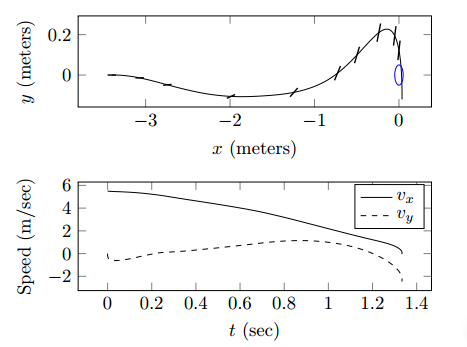
\includegraphics[scale=1]{gorodglide}
\caption{Optimal glide path with vertical and horizontal velocities \cite{Gorod}}
\label{gorodglide}
\end{figure}

The key to tensor-train value iterations success is the reduction in the number of states used. Of the $3.4 \times 10^{10}$ states making up the initial discretized state space, only about $10^6$ of these states are used as can be seen in \Cref{gorodstates}.\cite{Gorod}
\begin{figure}
\centering
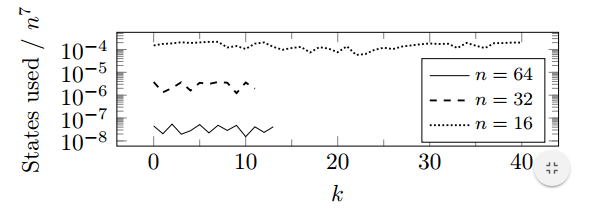
\includegraphics[scale=1]{gorodstates}
\caption{Fraction of states evaluated by TTVI in optimal glide problem \cite{Gorod}}
\label{gorodstates}
\end{figure}